\chapter{回溯法}

\section{算法思想} %%%%%%%%%%%%%%%%%%%%%%%%%%%%%%

当把问题分成若干步骤并递归求解时,如果当前步骤没有合法选择,则函数将返回上一级递归调用,
这种现象称为\textbf{回溯}(backtrack)。正是因为这个原因,枚举递归算法常被称为\textbf{回溯法}。

\textbf{回溯法 = 深搜 + 剪枝}。树的深搜或图的深搜都可以。深搜一般用递归来写,这样比较简洁。

回溯法比暴力枚举法快的原因,在于:暴力枚举法,是每生成一个完整的解答后,
再来判断这个解答是否合法,而回溯法则在生成每一步中都进行判断,
而不是等一个答案生成完毕后再来判断,这样,在每一步进行剪枝,减少了大量的废答案。

\section{八皇后问题} %%%%%%%%%%%%%%%%%%%%%%%%%%%%%%

\subsubsection{描述}
在8×8的棋盘上,放置8个皇后,使得她们互不攻击,每个皇后的攻击范围是
同行、同列和同对角线,要求找出所有解。如图~\ref{fig:eightQueens}所示。

\begin{center}
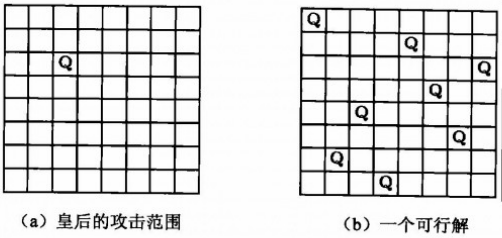
\includegraphics[width=240pt]{eight-queen.png} \\
\figcaption{八皇后问题}\label{fig:eightQueens}
\end{center}

\subsubsection{分析}
最简单的暴力枚举方法是,从64个格子中选一个子集,使得子集含有8个格子,且任意两个格子
都不在同一行、同一列或同一个对角线上。这正是子集枚举问题,然而64个格子的子集有$2^{64}$个,
太大了,这并不是一个很好的模型。

第二个思路是,从64个格子中选8个格子,这是组合生成问题。根据组合数学,有 $C_{64}^{8} \approx 4.426 \times 10^9$ 种方案,
比第一种方案优秀,但仍然不够好。

经过思考不难发现,由于每一行只能放一个皇后,那么第一行有8种选择,第二行有7中选择,…,
第8行有1中选择,总共有$8!=40320$个方案。如果用C[x]表示第x行皇后的列编号,则问题变成了一个
全排列生成问题,枚举量不会超过8!。

\subsubsection{代码}
\begin{Codex}[label=eight_queen.c]
#include <stdio.h>
#include <stdlib.h>

#define QUEENS 8 // 皇后的个数,也是棋盘的长和宽

int total = 0;	// 可行解的总数
int C[QUEENS];	// C[i]表示第i行皇后所在的列编号

/** 
 * @brief 输出所有可行的棋局,按列打印.
 *
 * http://poj.grids.cn/practice/2698/ , 这题需要按列打印
 *
 * @return 无
 */
void output() {
    int i, j;
    printf("No. %d\n", total);
    for (j = 0; j < QUEENS; ++j) {
        for (i = 0; i < QUEENS; ++i) {
            if (C[i] != j) {
                printf("0 ");
            } else {
                printf("1 ");
            }
        }
        printf("\n");
    }
}

/** 
 * @brief 输出所有可行的棋局,按行打印.
 * @return 无
 */
void output1() {
    int i, j;
    printf("No. %d\n", total);
    for (i = 0; i < QUEENS; ++i) {
        for (j = 0; j < QUEENS; ++j) {
            if (j != C[i]) {
                printf("0 ");
            } else {
                printf("1 ");
            }
        }
        printf("\n");
    }
}

/** 
 * @brief 检查当前位置(row, column)能否放置皇后.
 *
 * @param[in] row 当前行
 * @return 能则返回1,不能则返回0
 */
int check(const int row, const int column) {
    int ok = 1;
    int i;
    for(i = 0; i < row; ++i) {
        // 两个点的坐标为(row, column), (i, C[i])
        // 检查是否在同一列,或对角线上
        if(column == C[i] || row - i == column - C[i] || 
            row - i == C[i] - column) {
            ok = 0;
            break;
        }
    }
    return ok;
}

/** 
 * @brief 八皇后,回溯法
 *
 * @param[in] row 搜索当前行,该在哪一列上放一个皇后
 * @return 无
 */
void search(const int row) {
    if(row == QUEENS) {  // 递归边界,只要走到了这里,意味着找到了一个可行解
        ++total;
        output();
    } else {
        int j;
        for(j = 0; j < QUEENS; ++j) {  // 一列一列的试
            const int ok = check(row, j);
            if(ok) {  // 如果合法,继续递归
                C[row] = j;
                search(row + 1);
            }
        }
    }
}

// 表示已经放置的皇后
// 占据了哪些列
int columns[QUEENS];
// 占据了哪些主对角线
int principal_diagonals[2 * QUEENS];
// 占据了哪些副对角线
int counter_diagonals[2 * QUEENS];

/** 
 * @brief 检查当前位置(row, column)能否放置皇后.
 *
 * @param[in] row, 当前行
 * @return 能则返回1,不能则返回0
 */
int check2(const int row, const int column) {
    return columns[column] == 0 && principal_diagonals[row + column] == 0 
        && counter_diagonals[row - column + QUEENS] == 0;
}

/** 
 * @brief 八皇后,回溯法,更优化的版本,用空间换时间
 *
 * @param[in] row 搜索当前行,该在哪一列上放一个皇后
 * @return 无
 */
void search2(const int row) {
    if(row == QUEENS) {  // 递归边界,只要走到了这里,意味着找到了一个可行解
        ++total;
        output();
    } else {
        int j;
        for(j = 0; j < QUEENS; ++j) {  // 一列一列的试
            const int ok = check2(row, j);
            if(ok) {  // 如果合法,继续递归
                C[row] = j;
                columns[j] = principal_diagonals[row + j] = 
                    counter_diagonals[row - j + QUEENS] = 1;
                search2(row + 1);
                // 恢复环境
                columns[j] = principal_diagonals[row + j] = 
                    counter_diagonals[row - j + QUEENS] = 0;
            }
        }
    }
}

int main() {
    // search(0);
    search2(0);
    return 0;
}
\end{Codex}

\subsubsection{相关的题目}
与本题相同的题目:
\begindot
\item 《算法竞赛入门经典》\footnote{刘汝佳,算法竞赛入门经典,清华大学出版社,2009} 第123页7.4.1节
\item  百练 2698 八皇后问题, \myurl{http://poj.grids.cn/practice/2698/}
\myenddot

与本题相似的题目:
\begindot
\item POJ 1321 棋盘问题, \myurl{http://poj.org/problem?id=1321}
\myenddot


\section{还原IP地址} %%%%%%%%%%%%%%%%%%%%%%%%%%%%%%

\subsubsection{描述}
本题是 LeetCode Online Judge上的"Restore IP Addresses"。

给定一个只包含数字的字符串,还原出所有合法的IP地址。

例如:给定"25525511135",返回["255.255.11.135", "255.255.111.35"]。 (顺序无关紧要)

\subsubsection{分析}
这题很明显分为四步,有层次,因此可以尝试用回溯法解决。

\subsubsection{代码}
\begin{Codex}[label=restore_ip_adresses.cpp]
#include <iostream>
#include <vector>
using namespace std;

class Solution {
public:
    vector<string> restoreIpAddresses(string s) {
        vector<string> result;
        string ip;
        dfs(s, 0, 0, ip, result);
        return result;
    }

    /**
     * @brief 解析字符串
     * @param[in] s 字符串
     * @param[in] startIndex 从s的哪里开始
     * @param[in] step 当前步骤编号,从0开始编号,取值为0,1,2,3,4表示结束了
     * @param[in] intermediate 当前解析出来的中间结果
     * @param[out] result 存放所有可能的IP地址
     * @return 无
     */
    void dfs(string s, int startIndex, int step, string intermediate,
            vector<string> &result) {
        if (s.size() - startIndex > (4 - step) * 3)
            return;  // 非法结果,剪枝
        if (s.size() - startIndex < (4 - step))
            return;  // 非法结果,剪枝

        if (startIndex == s.size() && step == 4) {  // 找到一个合法解
            intermediate.resize(intermediate.size() - 1);
            result.push_back(intermediate);
            return;
        }

        int num = 0;
        for (int i = startIndex; i < startIndex + 3; i++) {
            num = num * 10 + (s[i] - '0');

            if (num <= 255) {  // 当前结点合法,则继续往下递归
                intermediate += s[i];
                dfs(s, i + 1, step + 1, intermediate + '.', result);
            }
            if (num == 0) {  // 非法结果,剪枝
                break;
            }
        }
    }
};
\end{Codex}


\section{Combination Sum} %%%%%%%%%%%%%%%%%%%%%%%%%%%%%%

\subsubsection{描述}
本题是 LeetCode Online Judge上的"Combination Sum"。

给定一个数的集合(C)和一个目标数(T),找到C中所有不重复的组合,让这些被选出来的数加起来等于T。

每一个数可以被选无数次。

注意:
\begindot
\item 所有的数(包括目标)都是正整数
\item 一个组合($a_1,a_2,\cdot,a_k$)中的元素必须以非递减顺序排列
\item 一个组合不能与另一个组合重复
\myenddot

例如,给定一组数2,3,6,7,和目标7,则答案是
\begin{Code}
[7]
[2, 2, 3] 
\end{Code}

\subsubsection{分析}
这题没有固定的步骤数,但是步骤也是有限的,因此可以尝试用回溯法。

\subsubsection{代码}

\begin{Codex}[label=combination_sum.cpp]
    vector<vector<int> > combinationSum(vector<int> &nums, int target) {
        std::sort(nums.begin(), nums.end());
        vector<vector<int> > result;
        vector<int> intermediate;
        dfs(nums, target, 0, intermediate, result);
        return result;
    }
    void dfs(vector<int>& nums, int gap, int level,
            vector<int>& intermediate, vector<vector<int> > &result) {
        if (gap == 0) {  // 找到一个合法解
            result.push_back(intermediate);
            return;
        }
        for (int i = level; i < nums.size(); i++) {
            if (gap < nums[i]) return; // 剪枝

            intermediate.push_back(nums[i]);
            dfs(nums, gap - nums[i], i, intermediate, result);
            intermediate.pop_back();  // 恢复环境
        }
    }
\end{Codex}


\section{Combination Sum II} %%%%%%%%%%%%%%%%%%%%%%%%%%%%%%

\subsubsection{描述}
本题是 LeetCode Online Judge上的"Combination Sum II"。

本题与上一题唯一不同的是,每个数只能使用一次。

\subsubsection{分析}
这题没有固定的步骤数,但是步骤也是有限的,因此可以尝试用回溯法。

\subsubsection{代码}
\begin{Codex}[label=combination_sum2.cpp]
    vector<vector<int> > combinationSum2(vector<int> &nums, int target) {
        sort(nums.begin(), nums.end());
        vector<vector<int> > result;
        vector<int> intermediate;
        dfs(nums, target, 0, intermediate, result);
        return result;
    }
    void dfs(vector<int> &nums, int gap, int index,
            vector<int> &intermediate, vector<vector<int> > &result) {
        if (gap == 0) {  //  找到一个合法解
            result.push_back(intermediate);
            return;
        }

        int previous = -1;
        for (int i = index; i < nums.size(); i++) {
            // 如果当前循环没有选nums[i],则下一次循环就不能再选nums[i]
            if (previous == nums[i])
                continue;
            if (gap < nums[i]) return;  // 剪枝

            previous = nums[i];

            intermediate.push_back(nums[i]);
            dfs(nums, gap - nums[i], i + 1, intermediate, result);
            intermediate.pop_back();  // 恢复环境
        }
    }
\end{Codex}
